\documentclass[a4paper,twoside,11pt]{article}
\usepackage[utf8]{inputenc}
\usepackage[english]{babel}
\usepackage{graphicx}
\usepackage{url}
\usepackage{float}

% pdflatex

% redefinição das margens das páginas
\setlength{\textheight}{24.00cm}
\setlength{\textwidth}{15.50cm}
\setlength{\topmargin}{0.35cm}
\setlength{\headheight}{0cm}
\setlength{\headsep}{0cm}
\setlength{\oddsidemargin}{0.25cm}
\setlength{\evensidemargin}{0.25cm}
\setlength{\textfloatsep}{16pt}

\begin{document}

\begin{figure}[t]
\centering

\includegraphics [width=5in]{logoISEL.png}
\end{figure}

\title{\huge \textbf{WaveCoach}\\[1ex]\LARGE Training Management Platform for Surf}

\author{
\begin{tabular}{c}
             Tiago Canilhas, n.º50472, e-mail: a50472@alunos.isel.pt, tel.: 924115540\\
             João Barrisco, n.º50476, e-mail: a50476@alunos.isel.pt, tel.: 967487235\\
\end{tabular}}

\date{
\begin{tabular}{ll}
  {Supervisor:} Filipe Freitas, e-mail: ffreitas@cc.isel.ipl.pt \\
\end{tabular}\\
\vspace{5mm}
April 28,  2025}

\maketitle

\section{Introduction}
The goal of this project is to develop a web application that allows the management of surfing athletes. This application is mainly aimed at coaches, but athletes can also access it to view their performance. Coaches will be able to register athletes, log different training sessions (e.g. gym, surf), record competition results, and monitor
performance through interactive charts. This will help them analyze progress and adjust training plans. This project is being developed to meet coaches' need for a more efficient and effective platform, replacing manual registration, which can be time-consuming and difficult to manage as the number of athletes grows. The platform not only saves time but also ensures greater accuracy and accessibility of data, allowing coaches to focus more on their athletes’ development and less on administrative tasks.

The project has already been initiated, and certain functionalities have already been developed, such as user registration, athlete management, and the athlete profile.

\section{Accomplished Tasks}


\subsection{Backend}

\subsubsection{Technologies}
\begin{itemize}
\item Kotlin
\item Spring Framework
\item Java Database Interface (JDBI)
\item PostgresSQL
\end{itemize}

\subsubsection{Entitity Relationship Model}

\begin{figure}[H]
\centering
\includegraphics[width=6in]{EA.png}
\caption{Entity Relationship Model}
\end{figure}

\subsubsection{Backend Organization}
\begin{figure}[H]
\centering
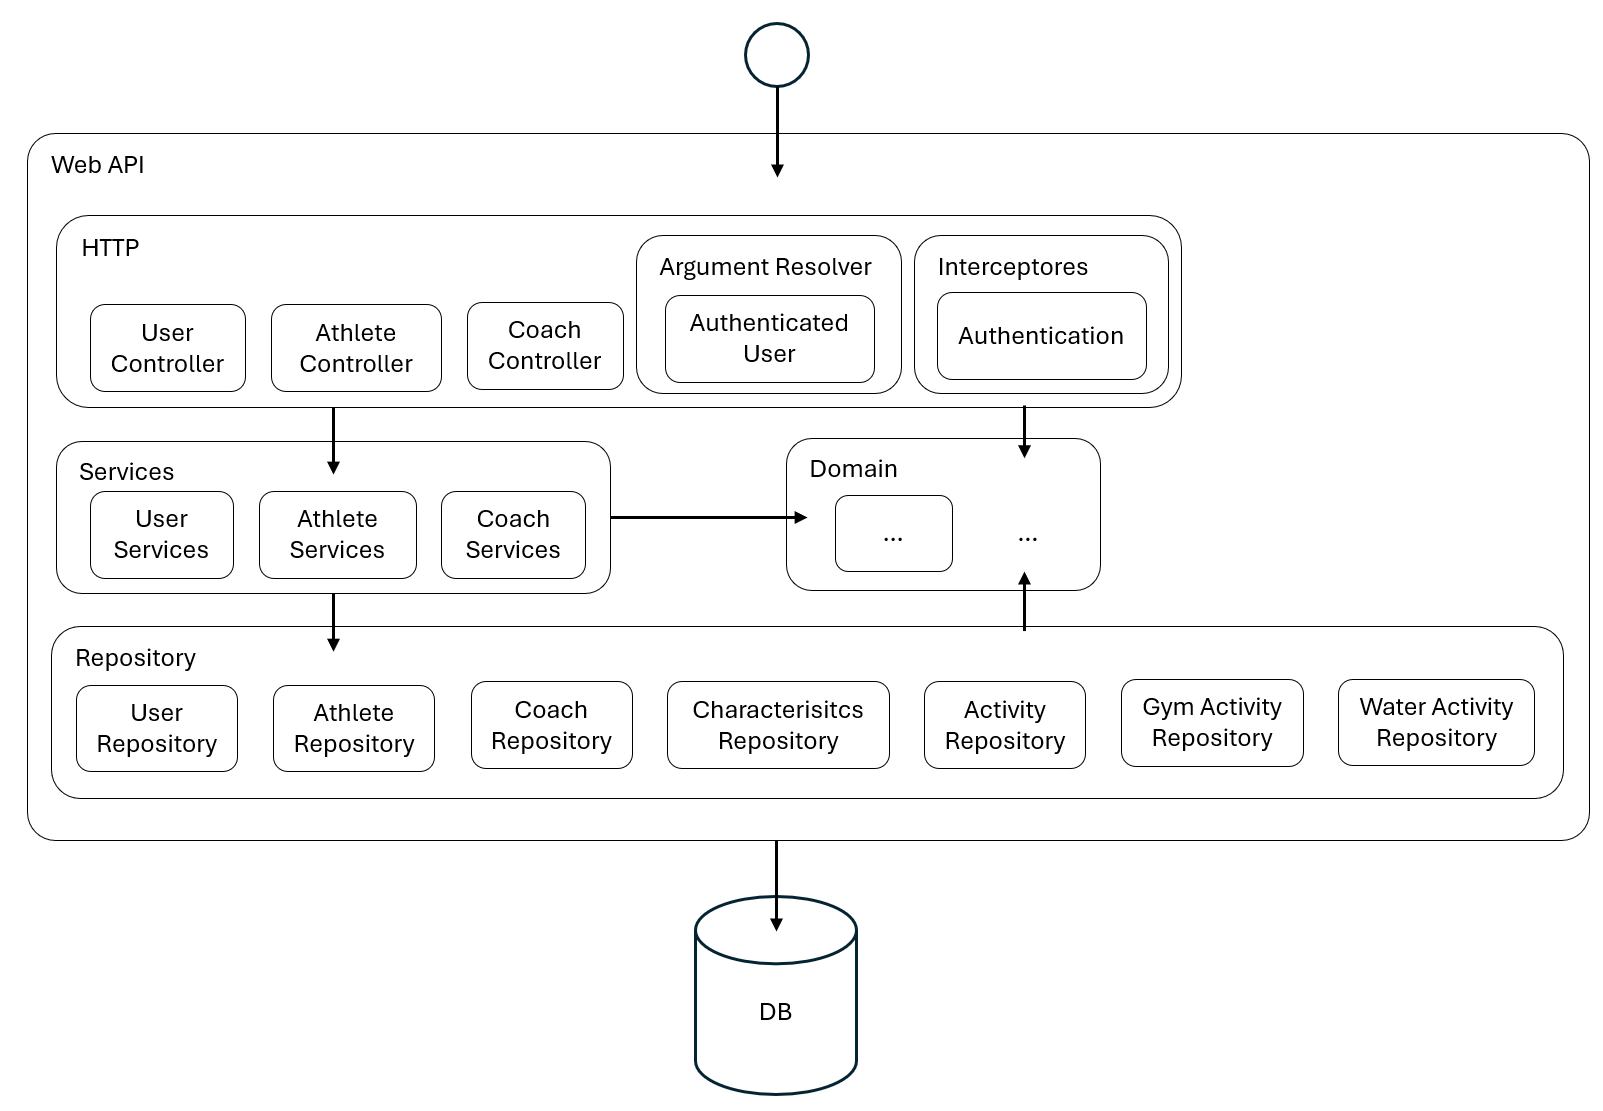
\includegraphics[width=5in]{BackendDiagram.png}
\caption{Backend Diagram}
\end{figure}

\subsubsection{Functionalities:}
\begin{itemize}
\item User Registration and Login - 
One of the first functionalities to be implemented was user registration. This is divided into two parts: athlete registration and coach registration. The athlete registration consists of two steps: first, the athlete enters a code that was provided by the coach, and second, the athlete adds their credentials, that is, a username and password. This process exists because our application is mainly aimed at coaches, meaning that, in order for coaches to easily and quickly add their athletes, the athletes do not need to have registered beforehand. Coach registration is simpler, requiring only a username and password. After the registration process was completed, the login functionality was then implemented.

No backend, para implementar estas funcionalidades... tendo sido, por fim, realizado testes para todas as funções criadas.

\item Athlete management - 
After user registration and login, aspects related to athlete management were developed, including the coach's functionalities to retrieve, add, update, and remove their athletes. All of these functionalities were thoroughly tested.

\item Athlete Profile - 
Finally, some functionalities related to the athlete were developed, such as the characteristics feature, where the functionalities to retrieve, add, update, and remove the athlete's characteristics were created and tested.

\end{itemize}

\subsection{Frontend}

\subsubsection{Technologies}
\begin{itemize}
\item Typescript
\item React
\item CSS Module
\item Webpack
\end{itemize}

\subsubsection{Frontend Organization}

\begin{figure}[H]
\centering
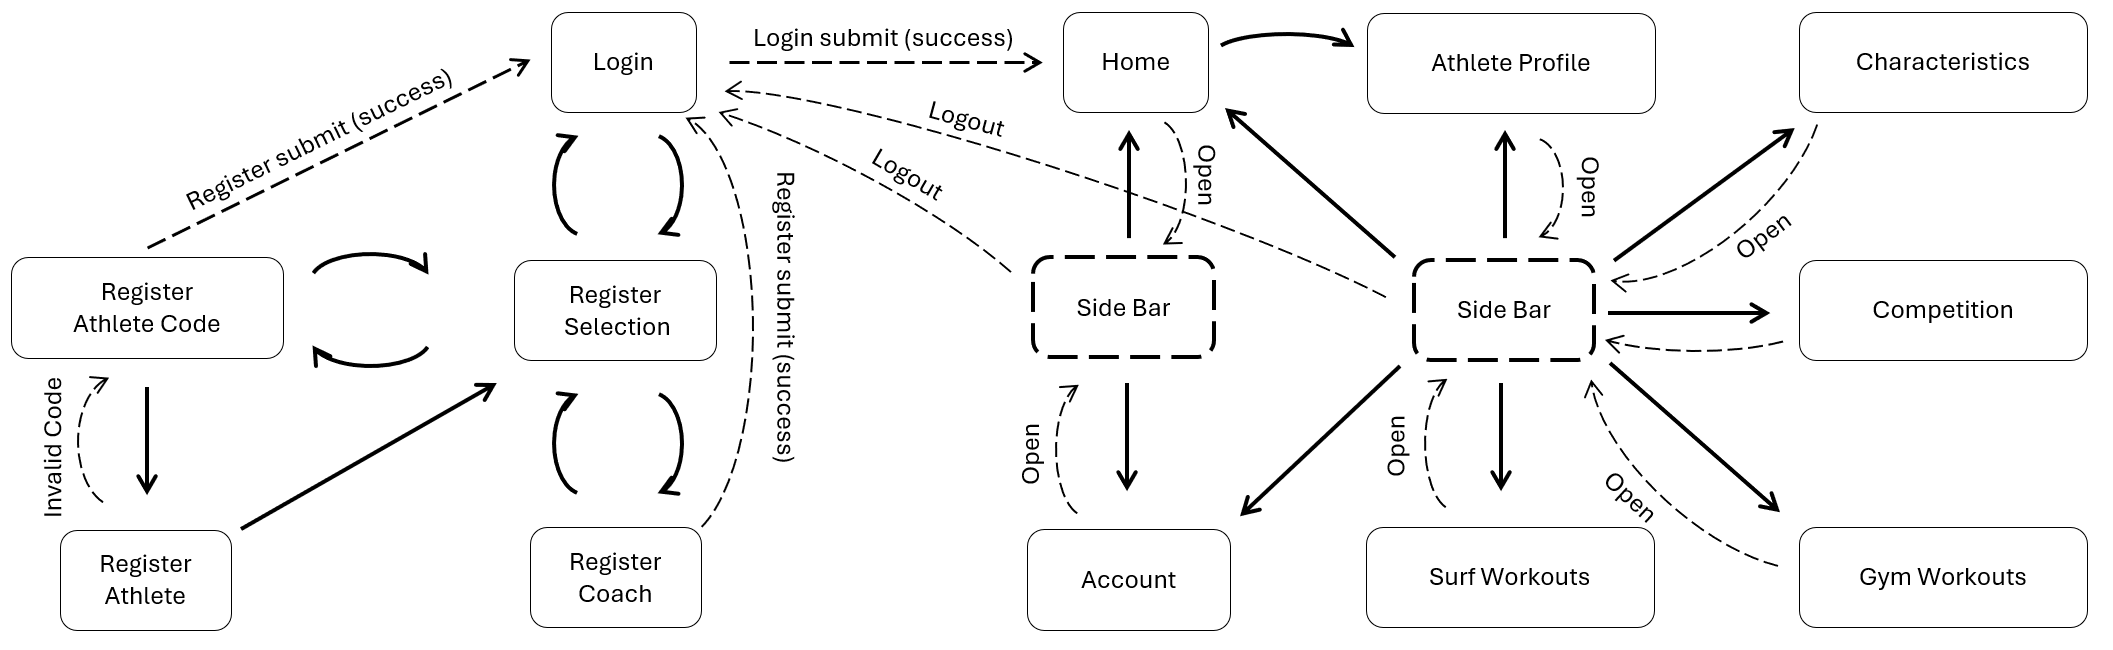
\includegraphics[width=5in]{ViewsDiagram.png}
\caption{Views Diagram}
\end{figure}

\subsubsection{Functionalities:}
\begin{itemize}
\item User Registration and Login - 
A primeira vista a ser realizada foi então a do login e a do registo, sendo esta, como anteriormente referido, diferente entre treinador e atleta.

\item Athlete management - 

\item Athlete Profile - 
The last view to be developed was the characteristics view. It consists of a chart where it is possible to visualize the athlete’s progress across different aspects, such as height, weight, calories, among others. The chart is clickable, and by clicking on it, users can view the characteristics for the selected date, where they can then edit or delete them. In addition to the chart, the view also displays the most recent characteristics, making it easier for the coach to quickly assess the athlete's current condition if they only need a quick overview.
\end{itemize}

\section{Pending Tasks}
At this stage, among the proposed functional requirements, the remaining tasks are the implementation of athlete training records, that is, water and gym trainings, athlete summaries, and competition records. In addition to these functionalities, an optional feature was also considered: a mobile app that would allow coaches to input athlete records more easily.

\begin{itemize}
\item Athletes' training records - For the implementation of the training records, both gym and water, it is necessary to create backend functionalities to retrieve, create, update, and delete trainings. On the frontend, two views need to be created, one for each type of training. The gym training view will include the record of the most recent training session, a table listing all gym trainings, where it will be possible to edit and delete them, and a button to add a new training session. In the water training view...

\item Athletes' summaries - 

\item Athletes' competition records - Para a implementação dos registos das competições, é tambem necessário 

\item Mobile App (new)
\end{itemize}

% \bibliographystyle{unsrt}
% \bibliography{references}

\end{document}